\documentclass[11pt,a4paper]{report}
\usepackage[utf8]{inputenc}
\usepackage[T1]{fontenc}
\usepackage{amsmath}
\usepackage{amsfonts}
\usepackage{amssymb}
\usepackage{graphicx}
\usepackage{float}
\usepackage{cleveref}

\newcommand{\dd}{\mathrm{d}}

\usepackage[a4paper, total={7in, 9.5in}]{geometry}

\begin{document}

\begin{center} 
\textbf{\Large Assignment 3} 
\end{center}

\begin{center}
\textbf{\Large Problem set 1 (60 marks)}
\end{center}

Consider a spring-mass system in \cref{fig:spring}. Let $k_i$, $i=1, 2, ..., 6$,  is the stiffness of spring $i$, $L_1, L_2, L_3, L_4, L_5$ are lengths of various springs at time $t=0$. Suppose $x_i = x_i(t)$, $i=1,2,3$, is the position of mass $m_i$ from the left wall at time $t$. 

Let $y_1 = x_1 - L_1$, $y_2 = x_2 - (L_1 + L_2)$, and $y_3 = x_3 - (L_1+L_2+L_4)$ are the displacements of the three masses at time $t$. Using the conservation of linear momentum principle, we arrive at the following linear system of second order ordinary differential equations:
\begin{align}\label{eq:ode}
m_1 \frac{\dd^2 y_1}{\dd t^2} &= -(k_1 + k_2 + k_3) y_1 + k_3 y_2, \notag \\
m_2 \frac{\dd^2 y_2}{\dd t^2} &= k_3 y_1 - (k_3 + k_4 + k_6) y_2 + k_4 y_3, \notag \\
m_3 \frac{\dd^2 y_3}{\dd t^2} &= k_4 y_2 - (k_4 + k_5) y_3, 
\end{align}

To solve the above coupled system of equations, we require total 6 initial conditions. We take:
\begin{align}\label{eq:ic}
y_1(0) = y_2(0) = y_3(0) = 0, \qquad \frac{\dd y_1}{\dd t}(0) = a, \quad \frac{\dd y_2}{\dd t}(0) = b, \quad \frac{\dd y_3}{\dd t}(0) = c .
\end{align}
Here, $a,b,c$ are the three given numbers.

\vspace{10pt}
\noindent\textit{Remark 1.} See the supplementary file `A3\_derivation\_spring\_system.pdf' for the derivation.

\vspace{10pt}
\noindent\textit{Parameters.} Let $k_1 = k_2 = k_4 = k_5 = 1$, $k_3 = k_6 = 2$, $m_3 = 1$, $m_1 = m_2 = 2$. Also, $a = 1$, $b=2$, and $c = -1$. 

\begin{figure}[H]
\centering
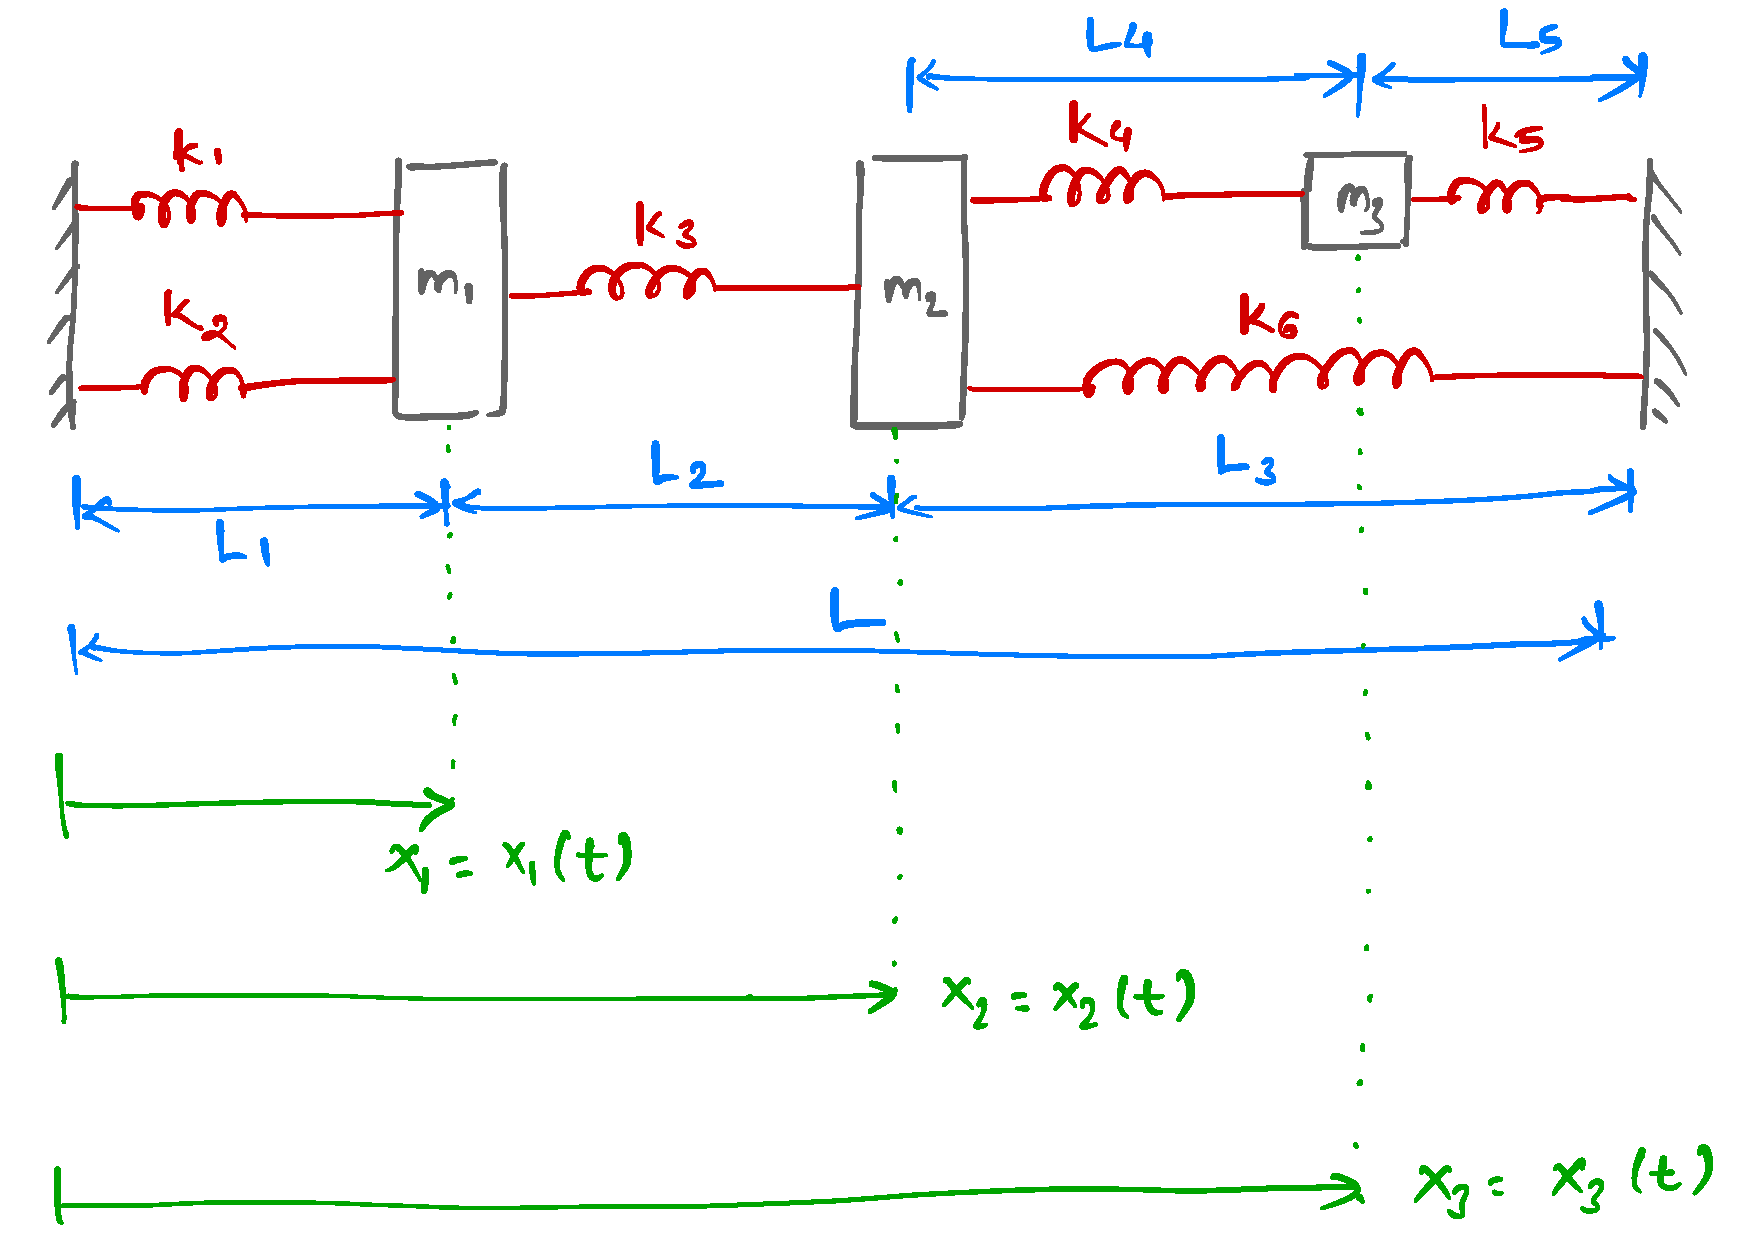
\includegraphics[width=0.6\textwidth]{spring_system_draw.pdf}
\caption{Spring-mass system.}\label{fig:spring}
\end{figure}

\vspace{10pt}
\noindent\textbf{Problem 1 (30 marks).} \textit{\textbf{Derive} characteristic (incomplete) solutions} of \cref{eq:ode}. Also, plot the three characteristics solutions separately between time interval $[0, 10]$. These three solutions show the three characteristics modes of vibration of spring-mass system.

\vspace{10pt}
\noindent\textbf{Problem 1 (30 marks).} \textit{\textbf{Find} the complete solution} that satisfies \cref{eq:ode} and \cref{eq:ic}.

\begin{center}
\textbf{\Large Problem set 2 (40 marks)}
\end{center}

Let $u_1 = u_1(t)$ and $u_2 = u_2(t)$ satisfies the following system of first order ordinary differential equation:
\begin{align}\label{eq:ode2}
\frac{\dd u_1}{\dd t} &= 3 u_1 + u_2, \notag \\
\frac{\dd u_2}{\dd t} &= -2 u_1 + 6 u_2 .
\end{align}

\vspace{10pt}
\noindent\textbf{Problem 1 (20 marks).} \textit{\textbf{Derive} characteristic (incomplete) solutions} of \cref{eq:ode2}.

\vspace{10pt}
\noindent\textbf{Problem 2 (10 marks).} Let $u_1, u_2$ also satisfies 
\begin{equation}\label{eq:ic2}
u_1(0) = a, \qquad u_2(0) = b,
\end{equation}
where $a, b$ are two parameters. 

\textit{\textbf{Find} the complete solution} that satisfies \cref{eq:ic2} for the two parameters $a$ and $b$. Clearly, the solution $u_1$ and $u_2$ will include $a$ and $b$.

\vspace{10pt}
\noindent\textbf{Problem 3 (10 marks).} Often times we deal with a situation where we observe system at specific time and want to know the state of system at past times. For example, we may want to know the value of $a$ and $b$ in \cref{eq:ic2} based on what we know about the solution $u_1$ and $u_2$ at some later time $T$. 

Using, $T = 10$,
\begin{equation}
u_1(10) = 1, \qquad u_2(10) = 2,
\end{equation}
\textit{\textbf{find} } the initial condition parameters $a$ and $b$. Use the solution $u_1$ and $u_2$ you obtained in \textbf{Problem 2}.


\end{document}